% =============================================================================
% SECTION 2: DATA DISCOVERY & EXPLORATORY DATA ANALYSIS
% =============================================================================
\section{Data Discovery \& Exploratory Data Analysis}

% ---------------- 4 DATA OVERVIEW ----------------
\begin{frame}{Dataset Characteristics Baseline}
\begin{columns}[c]
\column{0.55\textwidth}
\begin{block}{Dataset Structural Summary}
\begin{itemize}
    \item \textbf{Total Observations:} 10,000 corporate/retail records
    \item \textbf{Feature Space:} 17 predictors + 1 binary target
    \item \textbf{Target Metric:} \texttt{Exited} (0 = Retained, 1 = Churned)
    \item \textbf{Data Quality:} Zero missing values or null inputs detected
    \item \textbf{Problem Type:} Imbalanced Binary Classification
\end{itemize}
\end{block}

\column{0.45\textwidth}
\begin{exampleblock}{Core Analytical Scope}
Isolate underlying high-risk features and establish a production-ready model to predict individual attrition likelihood.
\end{exampleblock}
\end{columns}
\end{frame}

% ---------------- 5 DATA CHARACTERISTICS ----------------
\begin{frame}{Variable Typology Mappings}
\begin{columns}[T]
\column{0.48\textwidth}
\begin{block}{Continuous Numerical Metrics}
\begin{itemize}
    \item CreditScore, Age, Tenure
    \item Balance, EstimatedSalary
    \item Point Earned, Satisfaction Score
\end{itemize}
\end{block}

\column{0.48\textwidth}
\begin{block}{Categorical \& Binary Predictors}
\begin{itemize}
    \item Geography, Gender
    \item Card Type (Tiers)
    \item HasCrCard, IsActiveMember
    \item Complain (Historical Flag)
\end{itemize}
\end{block}
\end{columns}
\vspace{0.2cm}
\begin{alertblock}{Target Variable Boundary}
\texttt{Exited}: 0 representing active retention status vs. 1 indicating confirmed customer exit.
\end{alertblock}
\end{frame}

% ---------------- 6 CHURN DISTRIBUTION ----------------
\begin{frame}{Imbalanced Target Distribution}
\begin{columns}[c]
\column{0.55\textwidth}
\centering
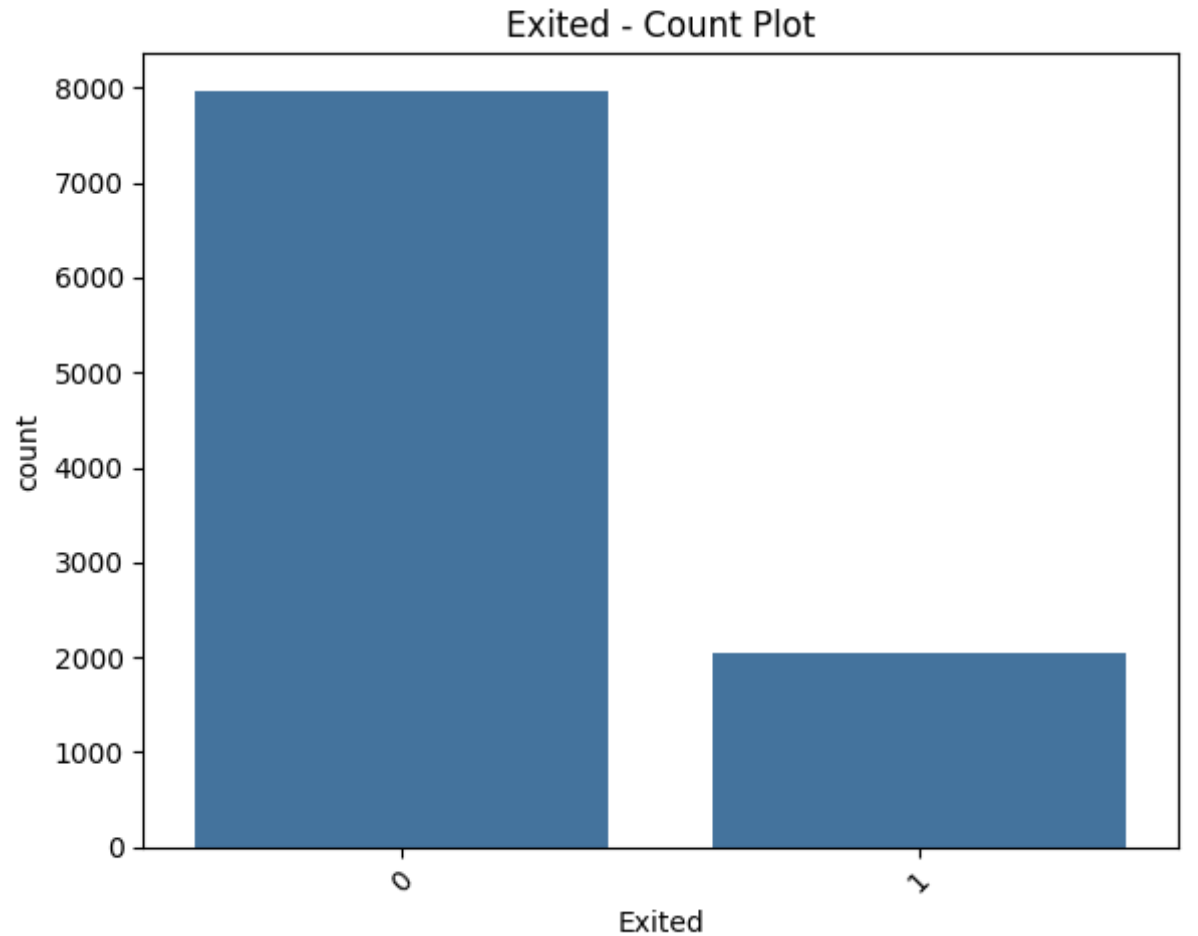
\includegraphics[width=0.85\linewidth]{figures/churn_distribution.png}

\column{0.45\textwidth}
\begin{block}{Statistical Diagnostics}
\begin{itemize}\scriptsize
    \item Baseline churn rate sits at approximately \textbf{20.3\%}.
    \item Class imbalance distorts standard accuracy metrics.
    \item Optimization relies strictly on Precision-Recall AUC (PR-AUC).
    \item Cost-sensitive adjustment implemented via XGBoost \texttt{scale\_pos\_weight}.
\end{itemize}
\end{block}
\end{columns}
\end{frame}

% ---------------- 7.1 EDA FINDINGS ----------------
\begin{frame}{EDA Insights: Customer Complaints Impact}
\begin{columns}[c]
\column{0.50\textwidth}
\centering
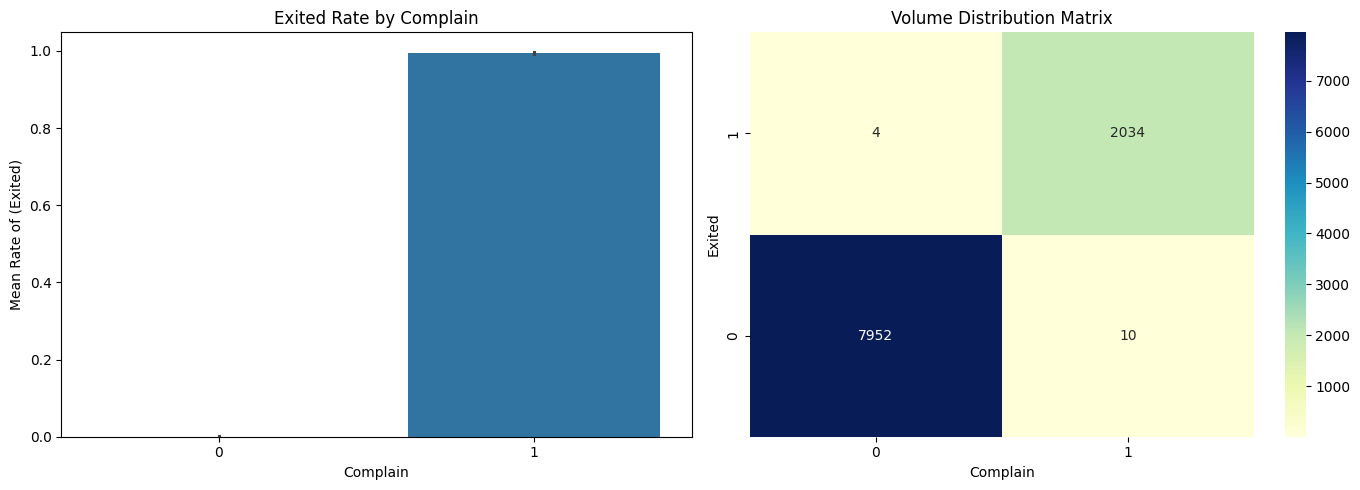
\includegraphics[width=\linewidth]{figures/complain_churn.png}

\column{0.50\textwidth}
\begin{alertblock}{Key Risk Vector}
Historical customer complaints show the strongest raw statistical association with ultimate customer exit.
\end{alertblock}
\begin{itemize}
    \item Unresolved service friction acts as an immediate attrition catalyst.
    \item Operationalizes customer service response time as a high-priority retention driver.
\end{itemize}
\end{columns}
\end{frame}

% ---------------- 7.2 EDA FINDINGS ----------------
\begin{frame}{EDA Insights: Product Density Trajectories}
\begin{columns}[c]
\column{0.50\textwidth}
\centering
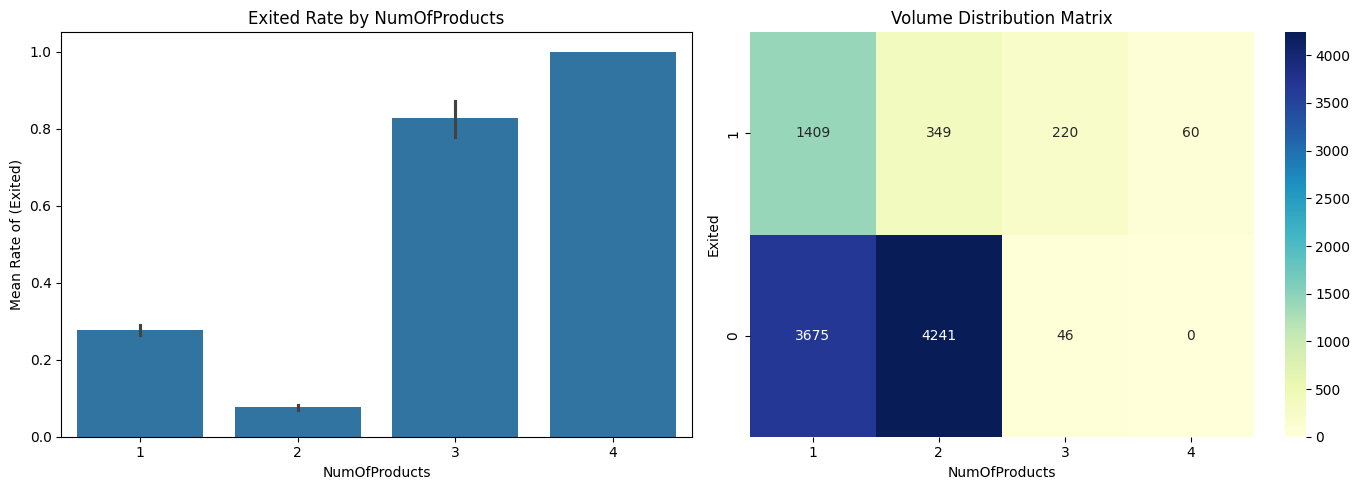
\includegraphics[width=\linewidth]{figures/products_churn.png}

\column{0.50\textwidth}
\begin{alertblock}{Product Congestion Anomaly}
Customers holding 3 or 4 products exhibit near-total churn rates.
\end{alertblock}
\begin{itemize}
    \item Core stability rests squarely at 1 or 2 products.
    \item High-density product portfolios signal cross-sell friction or misaligned accounts.
\end{itemize}
\end{columns}
\end{frame}

% ---------------- 7.3 EDA FINDINGS ----------------
\begin{frame}{EDA Insights: Macro Geographic Variations}
\begin{columns}[c]
\column{0.50\textwidth}
\centering
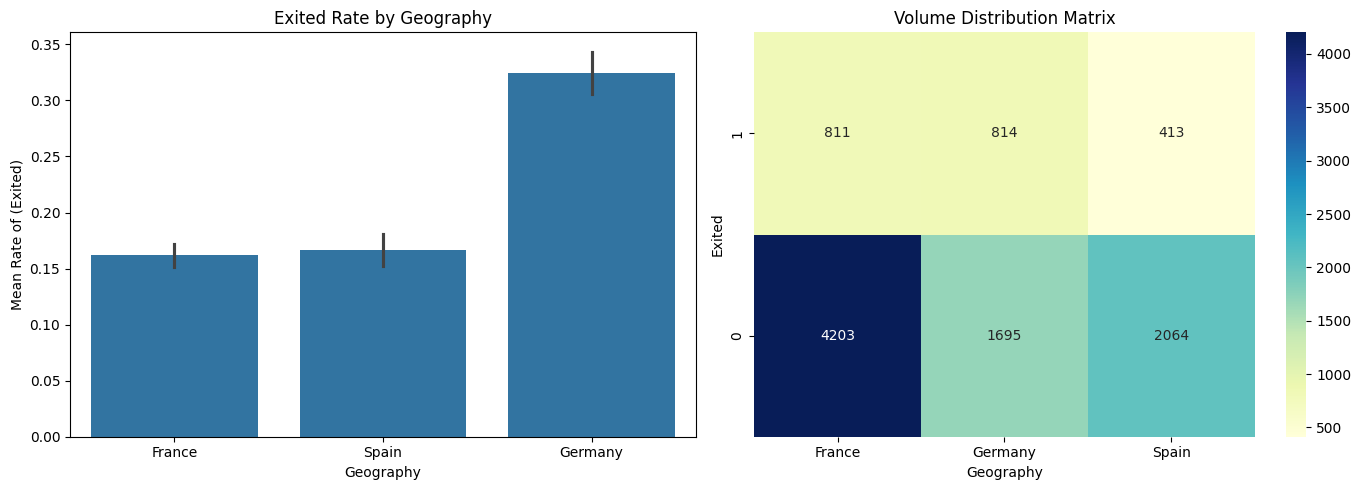
\includegraphics[width=\linewidth]{figures/geography_churn.png}

\column{0.50\textwidth}
\begin{alertblock}{Geographic Heterogeneity}
The churn rate in Germany is more than double the rates observed in France and Spain.
\end{alertblock}
\begin{itemize}
    \item Regional market variance points to localized competition or unique systemic constraints.
    \item Suggests a clear need for region-specific retention strategies.
\end{itemize}
\end{columns}
\end{frame}

% ---------------- 7.4 EDA FINDINGS ----------------
\begin{frame}{EDA Insights: Platform Engagement Footprint}
\begin{columns}[c]
\column{0.50\textwidth}
\centering
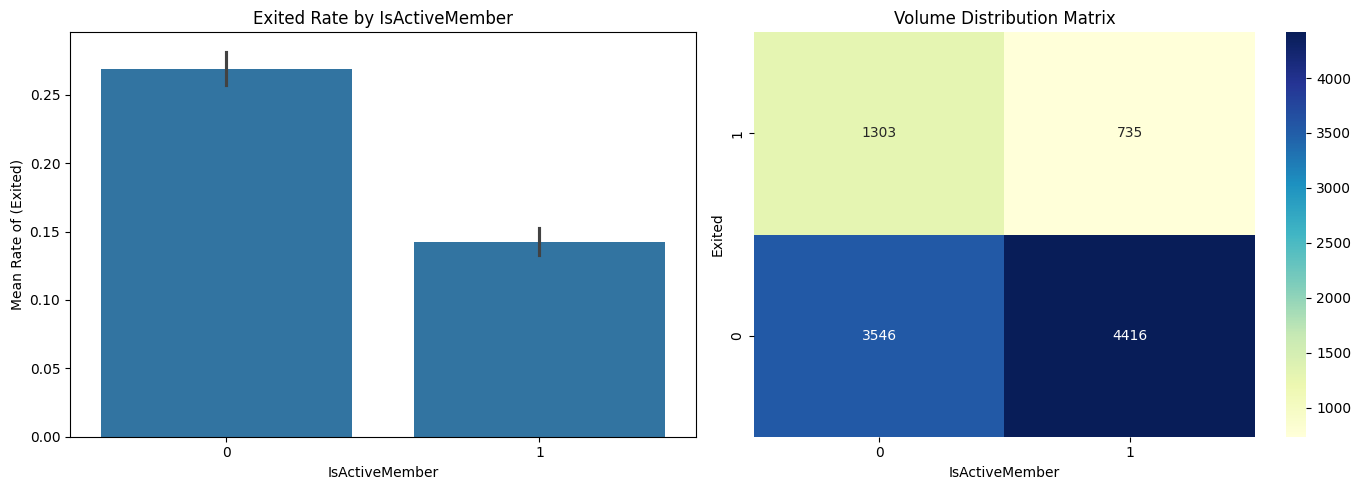
\includegraphics[width=\linewidth]{figures/active_churn.png}

\column{0.50\textwidth}
\begin{alertblock}{Engagement Variance}
Inactive account status heavily correlates with verified churn.
\end{alertblock}
\begin{itemize}
    \item Drop-offs in system usage serve as an early indicator of long-term attrition.
    \item Proactive re-engagement campaigns should focus on reviving slipping activity metrics.
\end{itemize}
\end{columns}
\end{frame}
